\begin{solution}
\begin{enumerate}
\item {[6 points]} If $v\in C^2_D(\Omega)$ and $w\in C^2_D(\Omega)$ then
\begin{eqnarray*}
\ip{Lv,w} &=& -\int_0^1 \int_0^1 \left(v_{xx}(x,y)+v_{yy}(x,y)\right) w(x,y)\,dx\,dy
\\
&=& -\int_0^1 \int_0^1 v_{xx}(x,y)w(x,y)\,dx\,dy-\int_0^1 \int_0^1 v_{yy}(x,y)w(x,y)\,dx\,dy
\\
&=& -\int_0^1 \int_0^1 v_{xx}(x,y)w(x,y)\,dx\,dy-\int_0^1 \int_0^1 v_{yy}(x,y)w(x,y)\,dy\,dx
\\
&=& -\int_0^1 \left(\left[v_x(x,y)w(x,y)\right]_{x=0}^{x=1}-\int_0^1 v_x(x,y)w_x(x,y)\,dx\right)\,dy
\\
&&-\int_0^1 \left(\left[v_y(x,y)w(x,y)\right]_{y=0}^{y=1}-\int_0^1 v_y(x,y)w_y(x,y)\,dy\right)\,dx
\\
&=& -\int_0^1 \left(\left[v_x(x,y)w(x,y)\right]_{x=0}^{x=1}-\left[v(x,y)w_x(x,y)\right]_{x=0}^{x=1}+\int_0^1 v(x,y)w_{xx}(x,y)\,dx\right)\,dy
\\
&&-\int_0^1 \left(\left[v_y(x,y)w(x,y)\right]_{y=0}^{y=1}-\left[v(x,y)w_y(x,y)\right]_{y=0}^{y=1}+\int_0^1 v(x,y)w_{yy}(x,y)\,dy\right)\,dx
\\
&=& -\int_0^1 \left(\left[v_x(x,y)w(x,y)\right]_{x=0}^{x=1}-\left[v(x,y)w_x(x,y)\right]_{x=0}^{x=1}\right)\,dy-\int_0^1\int_0^1 v(x,y)w_{xx}(x,y)\,dx\,dy
\\
&&-\int_0^1 \left(\left[v_y(x,y)w(x,y)\right]_{y=0}^{y=1}-\left[v(x,y)w_y(x,y)\right]_{y=0}^{y=1}\right)\,dx-\int_0^1\int_0^1 v(x,y)w_{yy}(x,y)\,dy\,dx
\\
&=& -\int_0^1 \left(\left[v_x(x,y)w(x,y)\right]_{x=0}^{x=1}-\left[v(x,y)w_x(x,y)\right]_{x=0}^{x=1}\right)\,dy-\int_0^1\int_0^1 v(x,y)w_{xx}(x,y)\,dx\,dy
\\
&&-\int_0^1 \left(\left[v_y(x,y)w(x,y)\right]_{y=0}^{y=1}-\left[v(x,y)w_y(x,y)\right]_{y=0}^{y=1}\right)\,dx-\int_0^1\int_0^1 v(x,y)w_{yy}(x,y)\,dx\,dy
\\
&=& -\int_0^1 \left(\left[v_x(x,y)w(x,y)\right]_{x=0}^{x=1}-\left[v(x,y)w_x(x,y)\right]_{x=0}^{x=1}\right)\,dy
\\
&&-\int_0^1 \left(\left[v_y(x,y)w(x,y)\right]_{y=0}^{y=1}-\left[v(x,y)w_y(x,y)\right]_{y=0}^{y=1}\right)\,dx
\\
&&-\int_0^1\int_0^1 v(x,y)\left(w_{xx}(x,y)+w_{yy}(x,y)\right)\,dx\,dy
\\
&=& -\int_0^1 \left(v_x(1,y)w(1,y)-v_x(0,y)w(0,y)-v(1,y)w_x(1,y)+v(0,y)w_x(0,y)\right)\,dy
\\
&&-\int_0^1 \left(v_y(x,1)w(x,1)-v_y(x,0)w(x,0)-v(x,1)w_y(x,1)+v(x,0)w_y(x,0)\right)\,dx
\\
&&+\ip{v,Lw}
\\
&=& \ip{v,Lw}
\end{eqnarray*}
since $w(1,y)=w(0,y)=v(1,y)=v(0,y)=w(x,1)=w(x,0)=v(x,1)=v(x,0)=0$ because $v,w\in C^2_D(\Omega)$. Consequently, $\ip{Lv,w}=\ip{v,Lw}\mbox{ for all }v,w\in C^2_D(\Omega)$.
\\
\item {[4 points]} We can compute that, for $j,k=1,2,\ldots$,
\begin{eqnarray*}
\left(L \psi_{j,k}\right)(x,y) &=& -{\partial^2 \over \partial x^2} \left(2\sin(j\pi x)\sin(k\pi y)\right)-{\partial^2 \over \partial y^2} \left(2\sin(j\pi x)\sin(k\pi y)\right)
\\
&=& 2j^2\pi^2 \sin(j\pi x)\sin(k\pi y)+2k^2 \pi^2 \sin(j\pi x)\sin(k\pi y)
\\
&=& 2\left(j^2 + k^2\right)\pi^2 \sin(j\pi x)\sin(k\pi y)
\\
&=& \left(j^2 + k^2\right)\pi^2\psi_{j,k}(x,y).
\end{eqnarray*}
Hence,
\[
\lambda_{j,k}=(j^2+k^2)\pi^2\mbox{ for }j,k=1,2,\ldots.
\]
\\
\item {[7 points]} The operator $L_1$ has eigenfunctions $\psi_p$ for $p=1,2,3,\ldots$ which are such that
\[
\psi_p(s)=\sqrt{2}\sin(p\pi s)
\]
for $p=1,2,3,\ldots$ and
\[
 \int_0^1 \psi_p(s)\psi_q(s)\, ds=\left\{\begin{array}{ll} 1 & \mbox{if }p=q \\ 0 & \mbox{if }p\ne q \end{array}\right.
\]
for $p,q=1,2,3,\ldots$. Therefore,
\begin{eqnarray*}
\ip{\psi_{j,k}, \psi_{m,n}} &=& \int_0^1 \int_0^1 2\sin(j\pi x) \sin(k\pi y) 2\sin(m\pi x) \sin(n\pi y)\,dx\,dy
\\
&=& \int_0^1 \int_0^1 \psi_j(x) \psi_k(y) \psi_m(x) \psi_n(y) \,dx\,dy
\\
&=& \int_0^1 \psi_k(y) \psi_n(y) \int_0^1 \psi_j(x) \psi_m(x) \,dx\,dy
\\
&=& \left\{\begin{array}{ll} \displaystyle{\int_0^1 \psi_k(y) \psi_n(y) \,dy} & \mbox{if }j=m \\ \displaystyle{0} & \mbox{if }j\ne m \end{array}\right.
\\
&=& \left\{\begin{array}{ll} 1 & \mbox{if }j=m\mbox{ and }k=n \\ 0 & \mbox{otherwise} \end{array}\right.
\end{eqnarray*}
for $j,k,m,n=1,2,3,\ldots$.
\\
\item {[8 points]} The requested plots and the code used to produce them are below.

      \begin{center} 
          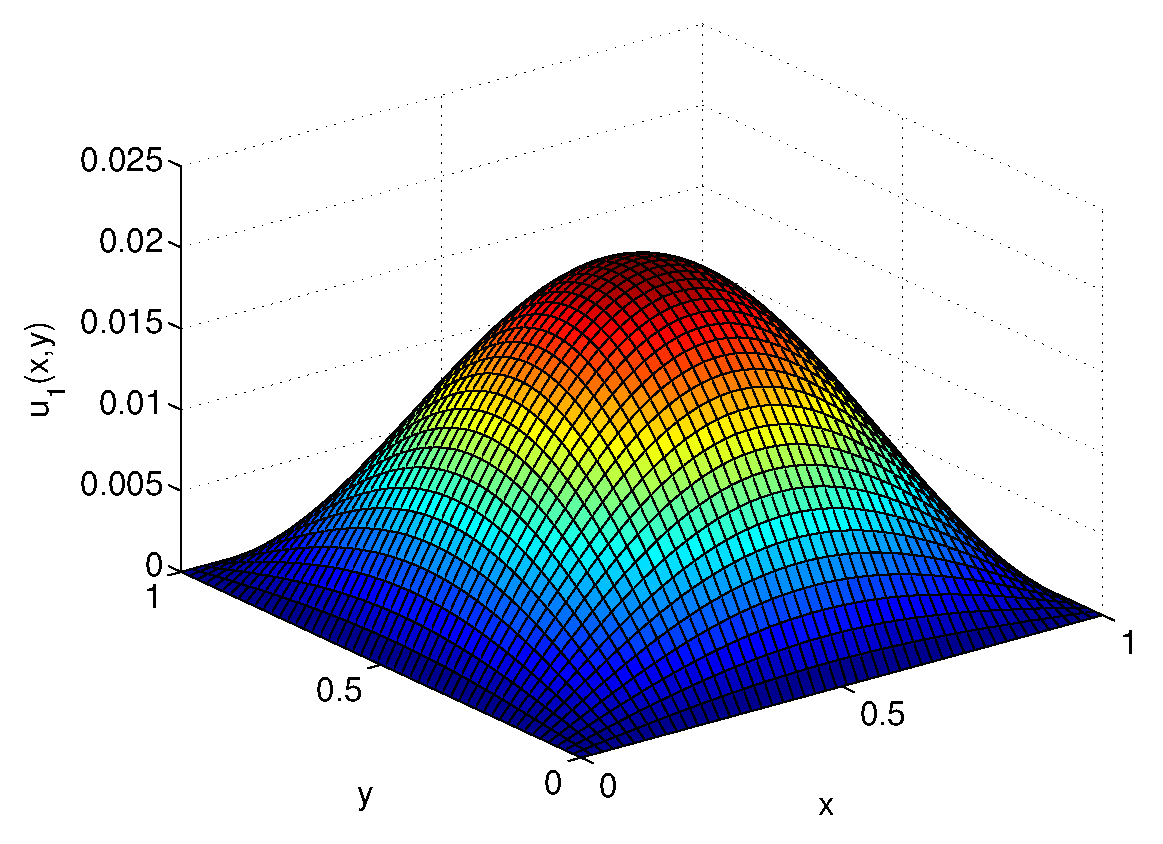
\includegraphics[scale=0.37]{twoD1}\quad
          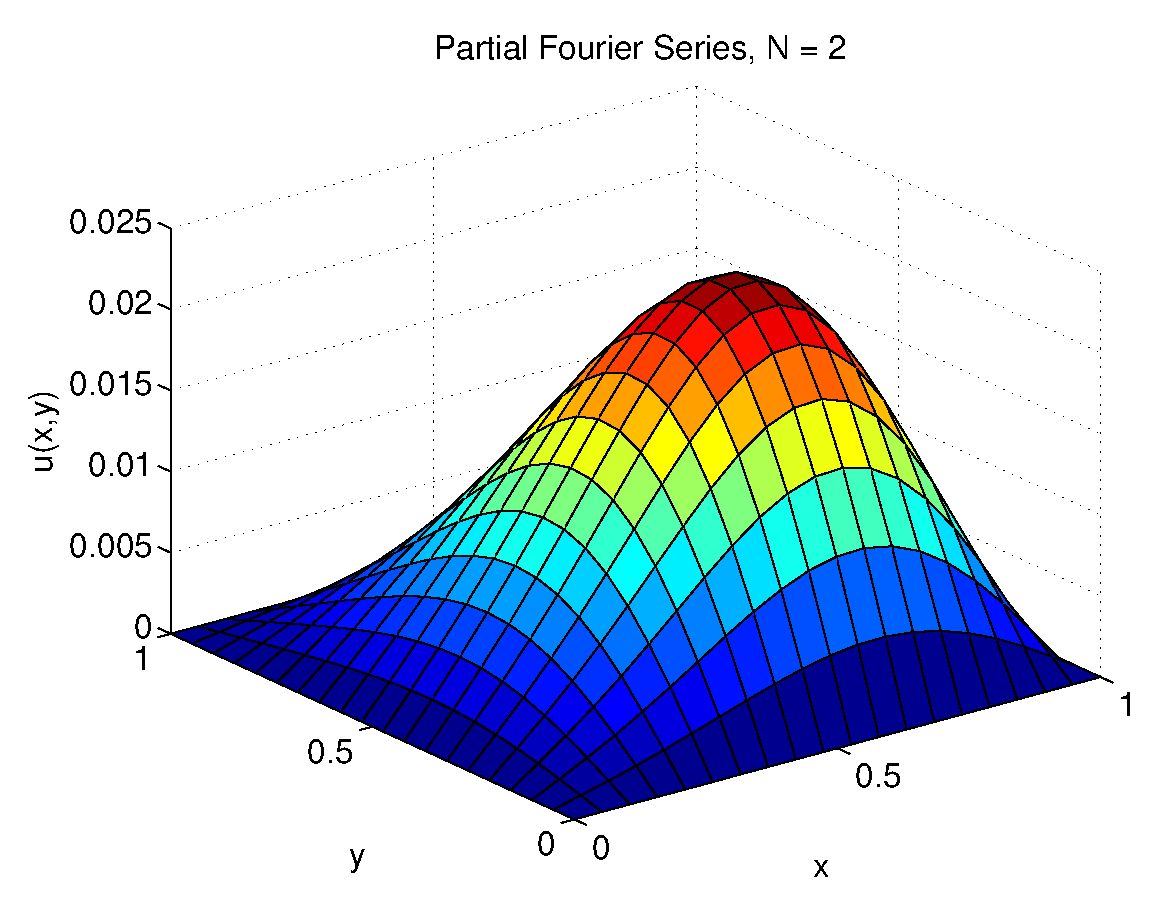
\includegraphics[scale=0.37]{twoD2}

          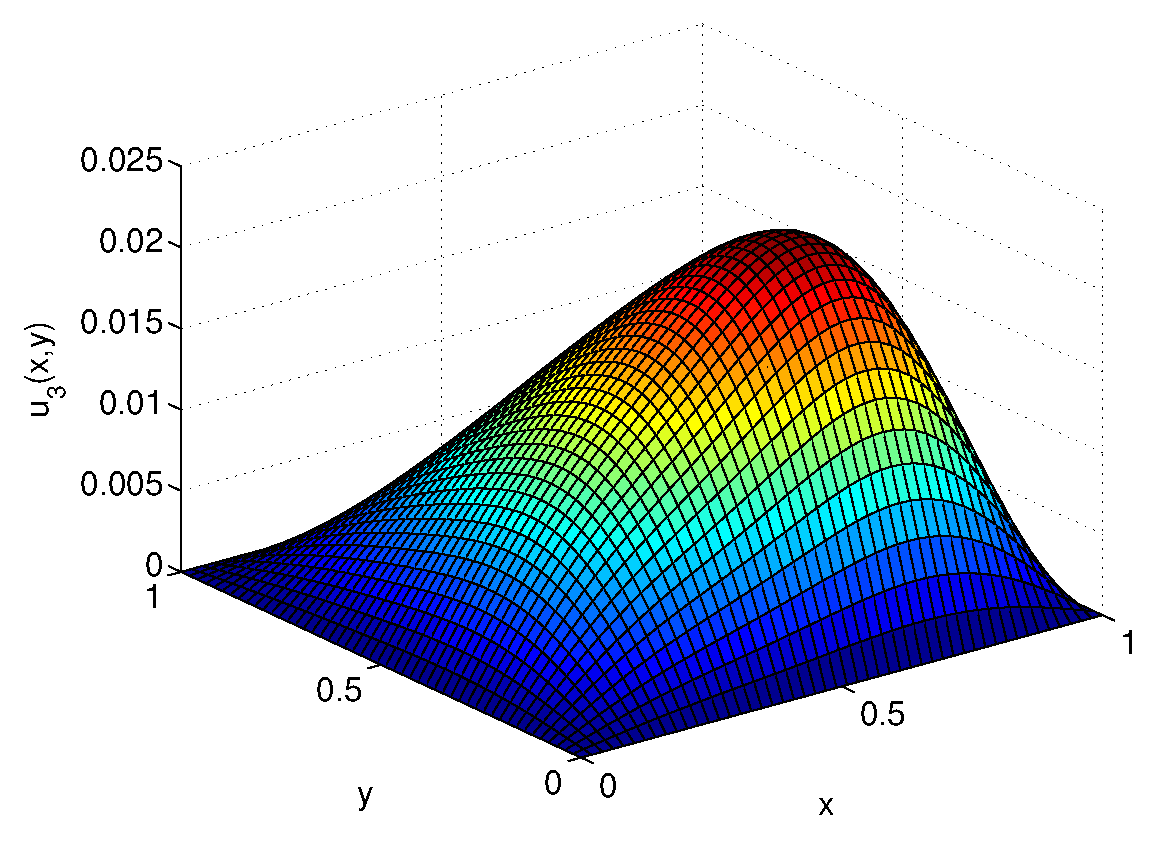
\includegraphics[scale=0.37]{twoD3}\quad
          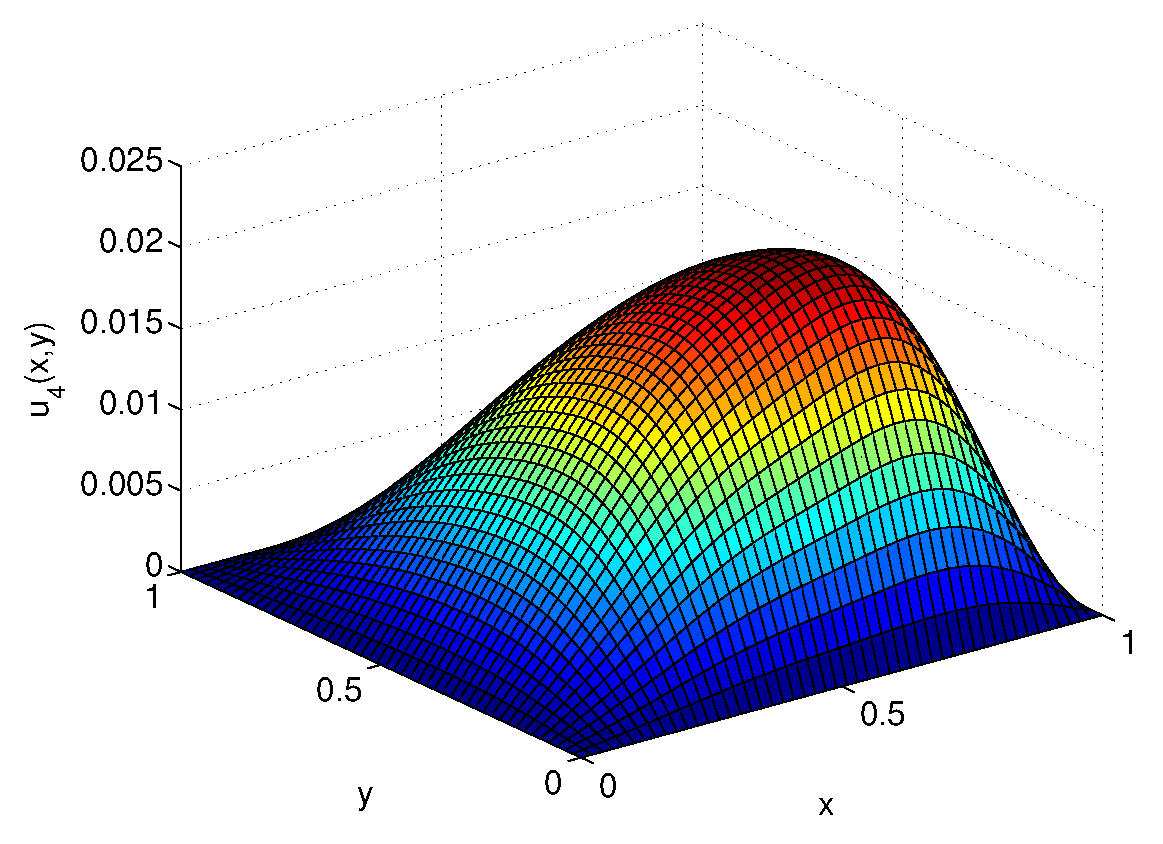
\includegraphics[scale=0.37]{twoD4}

          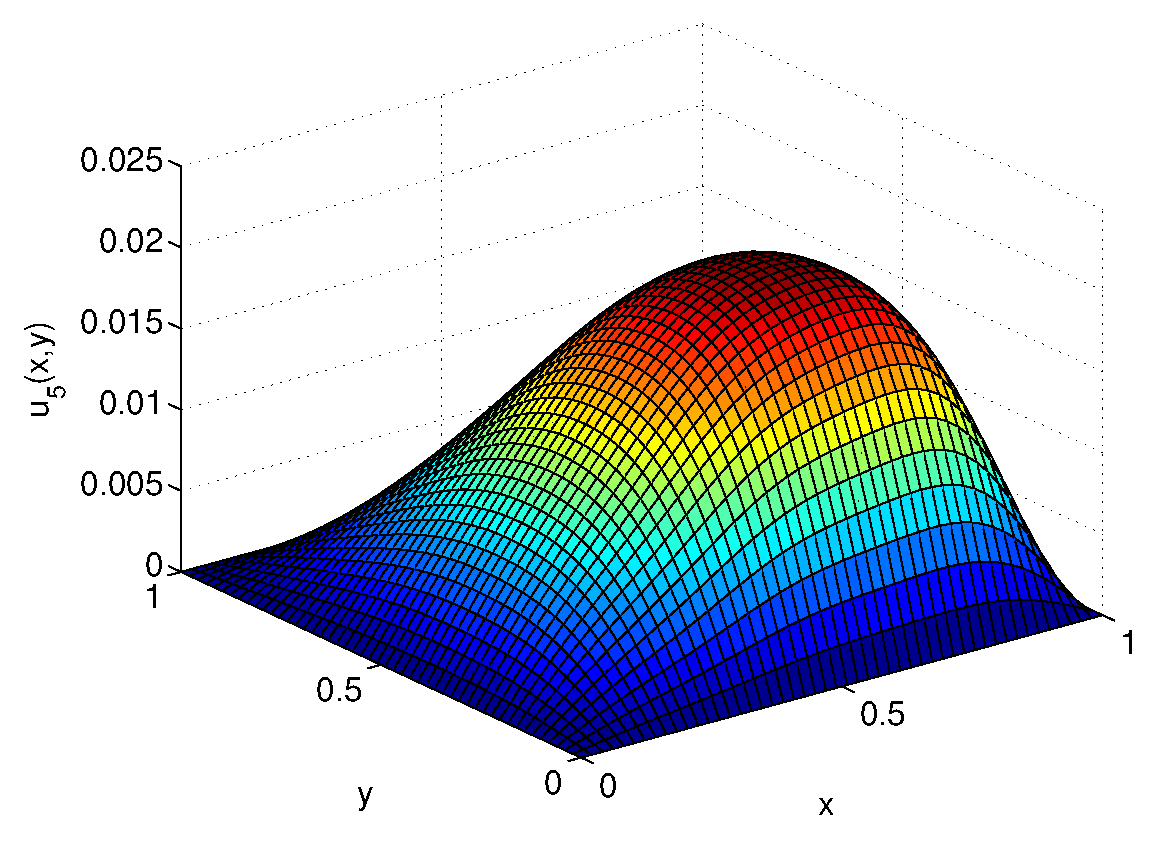
\includegraphics[scale=0.37]{twoD5}\quad
          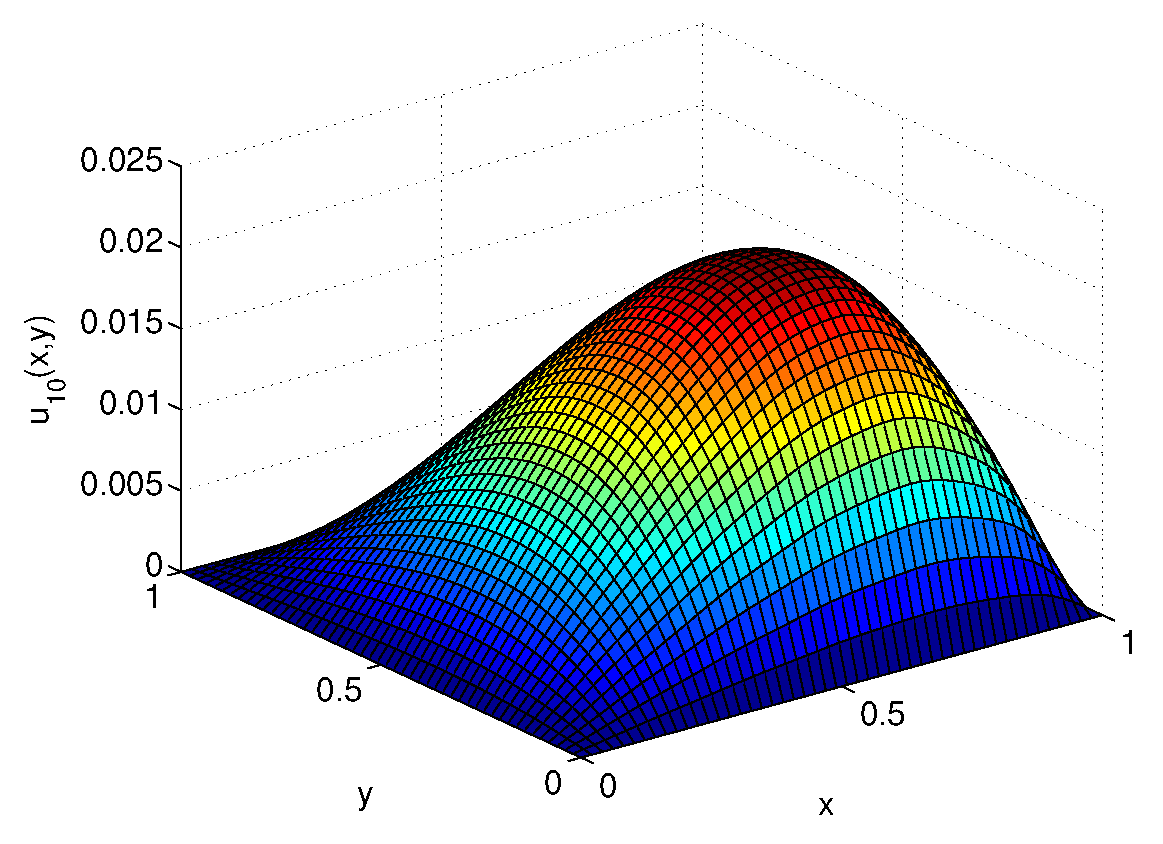
\includegraphics[scale=0.37]{twoD10}
      \end{center}

\lstinputlisting{HW42.m}

\end{enumerate}
\end{solution}